\chapter{Textos y formatos} \label{se:EPT} 

El tipo de fichero básico con el que trabajan los profesionales de la traducción suele ser un fichero con texto, es decir, un texto informatizado, también llamado \emph{documento de texto}. Este fichero puede contener, además del texto mismo, información sobre la presentación (el formato de los párrafos y de las páginas, los tipos y los tamaños de letra que se usan con cada palabra, etc.) o sobre la organización del contenido (indicaciones de que una determinada parte del texto es el título de un capítulo, el título de una sección o una nota a pie de página, etc.). 

Un texto informatizado puede tener diversos orígenes: \begin{itemize} \item Puede haber sido generado por otro programa de ordenador, por ejemplo a partir de los datos contenidos en alguna base de datos (véase el capítulo~\ref{se:basesdades}). \item Lo podemos haber recibido anexo a un mensaje de correo electrónico (véase el apartado~\ref{ss:correue}) o por mensajería instantánea (véase el apartado~\ref{ss:missinst}). \item Lo podemos haber descargado (copiado) de algún servidor de Internet (veáse la pág. \pageref{pg:ftp}). \item Lo podemos haber generado, quizás a partir de otro texto, usando un \emph{procesador de textos} (veáse el apartado \ref{ss:proctext}). \item Lo puede haber generado un \emph{sistema de reconocimiento del habla} a partir de la voz de la persona que lo ha dictado. \item Lo puede haber generado un \emph{sistema de reconocimiento de textos escritos} a partir de un texto tipografiado o manuscrito. \end{itemize} 

%%%%%%%%%%%%%
\section{Formatos de texto} \label{ss:formats} Un \emph{texto informatizado} es, como cualquier porción de datos informatizada, una \emph{secuencia de bits}, es decir, de \emph{unos} y \emph{ceros}, del estilo de la siguiente:  \begin{center} \texttt{010000010100110101001001\ldots} \end{center} 

Como ya hemos visto en el apartado~\ref{ss:memoria}, los \emph{bits} se agrupan en grupos de ocho (\emph{bytes}): \begin{center} \texttt{01000001 01001101 01001001\ldots} \end{center} 

Hay muchas maneras de organizar estos bytes para almacenar los textos; muchos de los problemas que aparecen cuando se tratan textos con el ordenador provienen de discrepancias en cuanto a la manera de hacerlo. 
En las siguientes secciones estudiaremos dos aspectos importantes que denominaremos \emph{codificación} y \emph{formato} propiamente dicho. La \emph{codificación} es la asignación de una secuencia concreta, de uno o más \emph{bytes}, a cada posible carácter de un texto. El \emph{formato} de un documento es la parte no textual de este y sirve para codificar información estructural (sobre la organización del contenido del documento) o presentacional (sobre la apariencia que tendrá el documento cuando se presente). 

\section{Codificación de caracteres} La codificación de los caracteres de un texto consta de dos fases: \begin{enumerate} \item Se asigna a cada carácter un número entero positivo llamado \emph{punto de código} o simplemente \emph{código}; por ejemplo: ``\texttt{a}'' $\to$ 97; ``\texttt{?}'' $\to$ 63. \item los códigos numéricos se convierten en bytes asignándoles una determinada secuencia de bits; por ejemplo: 97 $\to$ \texttt{01100001}; 63 $\to$ \texttt{00111111}. 

% Esta fase de vegades s'anomena \emph{serialització}.
\end{enumerate} 

\subsection{ASCII} Como ya se ha comentado en la página~\pageref{pg:ASCII}, para almacenar textos se ha usado históricamente el estándar ASCII (\emph{American Standard Code for Information Interchange}). Este estándar asigna un número del 0 al 127 a cada carácter del alfabeto latino usado en inglés y usa 7 bits para codificarlo,\footnote{Con 7 bits se pueden hacer $2^7=128$ combinaciones. Por eso, los códigos asignados por ASCII van del 0 al 127.} de forma que permite almacenar un carácter por byte y todavía sobra un bit.\footnote{Inicialmente este bit se usaba como bit de control para detectar errores en la transmisión de los textos.} La tabla~\ref{tb:ASCII} muestra algunos ejemplos de códigos ASCII. Los códigos ASCII del 0 al 31 no corresponden a caracteres imprimibles sino a \emph{caracteres de control} que tienen nombres especiales y se usan para un control rudimentario del formato y de la transmisión de los textos. 

\begin{table} \begin{center} \begin{tabular}{c|l|l} \hline\hline \textsc{Código binario} &\textsc{código decimal} &\textsc{carácter} \\ \hline

\texttt{0000000} &0 &NUL (carácter nulo) \\ $\cdots$ &$\cdots$ &$\cdots$ \\ \texttt{0001001} &9 &TAB (tabulador) \\ \texttt{0001010} &10 &NL (nueva línea) \\ $\cdots$ &$\cdots$ &$\cdots$ \\ \texttt{0001101} &13 &CR (retorno de carro) \\ $\cdots$ &$\cdots$ &$\cdots$ \\ \texttt{0100000} &32 &(un espacio en blanco) \\ \texttt{0100001} &33 &\texttt{!} \\ \texttt{0100010} &34 &\verb+"+ \\ $\cdots$ &$\cdots$ &$\cdots$ \\ \texttt{0110000} &48 &\texttt{0} \\ \texttt{0110001} &49 &\texttt{1} \\ $\cdots$ &$\cdots$ &$\cdots$ \\ \texttt{0111000} &56 &\texttt{8} \\ \texttt{0111001} &57 &\texttt{9} \\ $\cdots$ &$\cdots$ &$\cdots$ \\ \texttt{1000000} &64 &\texttt{@} \\ \texttt{1000001} &65 &\texttt{A} \\ \texttt{1000010} &66 &\texttt{B} \\ $\cdots$ &$\cdots$ &$\cdots$ \\ \texttt{1011010} &90 &\texttt{Z} \\ \texttt{1011011} &91 &\texttt{[} \\ $\cdots$ &$\cdots$ &$\cdots$ \\ \texttt{1100000} &96 &\verb+`+ \\ \texttt{1100001} &97 &\texttt{a} \\ \texttt{1100010} &98 &\texttt{B} \\ $\cdots$ &$\cdots$ &$\cdots$ \\ \texttt{1111010} &122 &\texttt{z} \\ \texttt{1111011} &123 &\verb+{+ \\ $\cdots$ &$\cdots$ &$\cdots$ \\ \texttt{1111110} &126 &\verb+~+ \\ \end{tabular} \end{center} \caption{Algunos ejemplos del código ASCII. Los códigos del 0 al 31 no corresponden a caracteres imprimibles sino a caracteres de control.} \label{tb:ASCII} \end{table} 

El estándar ASCII tiene la limitación de que no permite escribir caracteres propios de muchas lenguas europeas, como, por ejemplo, letras con signos diacríticos (\emph{á}, \emph{ò}, \emph{ç}, \emph{ñ}, \emph{ü}, etc.) o letras especiales como \emph{ß}. 

\subsection{Extensiones de ASCII} \label{s3:ISO} Con la llegada de los microordenadores\footnote{Los primeros ordenadores que tenían un tamaño que permitía tener uno en casa.} en los años ochenta se decidió ampliar el estándar ASCII, de 7 bits y por lo tanto con $2^7=128$ caracteres diferentes, a un código de 8 bits con $2^8=256$ caracteres diferentes. El octavo bit o ``bit 7''\footnote{Recordad que en informática es habitual contar empezando por el cero.}---el primero por la izquierda--- es 1 para los nuevos caracteres (numerados del 128 al 255) y cero para los caracteres estándares de ASCII. 

Hay varias extensiones de ASCII, cada una dirigida a un conjunto de lenguas concreto que usan (casi) el mismo alfabeto. En nuestra área geográfica se usa normalmente la codificación ISO-8859-1 o \emph{Latin-1} (véase la tabla~\ref{tb:ISO88591}); esta codificación sirve para las lenguas siguientes: \emph{afrikaans} (lengua germánica hablada en la República Sudafricana), alemán, inglés, vasco, catalán, danés, escocés, español, feroés, finés, francés, gallego, irlandés, islandés, italiano, neerlandés, noruego, portugués y sueco.\footnote{Hay una modificación llamada ISO-8859-15, que incluye, entre otros, el símbolo del euro y resuelve algunos problemas referentes al francés y al finés.} El sistema operativo Windows de Microsoft usa la codificación de 8 bits denominada CP-1252, también llamada \emph{WinLatin-1}, que es más amplia que ISO-8859-1, puesto que usa algunos de los códigos 128--159 para caracteres (por ejemplo, usa el código 128 para el símbolo del euro). 

Hay otras codificaciones en la familia ISO-8859. Por ejemplo, el albanés, el bosnio, el croata, el checo, el húngaro y el rumano usan una codificación llamada ISO-8859-2 o \emph{Latin-2}; el letón, el lituano y el estonio usan la ISO-8859-4 o \emph{Latin 4}; el ruso usa la ISO-8859-5 que contiene el alfabeto cirílico además del alfabeto latino básico. Por eso, es muy importante conocer qué esquema de codificación de caracteres se ha usado en un documento de texto determinado para poderlo leer correctamente; algunos formatos de texto incluyen esta información dentro del mismo documento. 

El hecho de que haya varias maneras de usar los nuevos códigos hace que a veces los textos con caracteres especiales no queden bien cuando pasamos de un procesador de textos (o un editor de textos) a otro (los caracteres de ASCII se ven normalmente bien: los que fallan son los nuevos). Fijaos en que si en un documento ISO-8859-1 se escribe la frase \emph{Què és això?}, donde los caracteres ``\texttt{è}'', ``\texttt{é}'' y ``\texttt{ò}'' tienen códigos por encima de 127 (233, 232 y 242 respectivamente), e intentamos leerlo como si fuera un documento ISO-8859-2, leeremos \emph{>Quč és aixň?}, porque dos de estos códigos (233 y 242) tienen otra interpretación en esta codificación (``\texttt{č}'' y ``\texttt{ň}'' respectivamente). Por ello, no podemos mezclar en un mismo documento textos en lenguas que usan extensiones de ASCII diferentes. 

\begin{table} \begin{center} \begin{tabular}{c|l|l} \hline\hline \textsc{Código binario} &\textsc{código decimal} &\textsc{carácter} \\ \hline

\texttt{10100000} &160 &(espacio no rompible) \\ \texttt{10100001} &161 &\texttt{¡} \\ $\cdots$ &$\cdots$ &$\cdots$ \\ \texttt{10110101} &181 &$\mathtt{\mu}$ \\ \texttt{10110110} &182 &\texttt{¶} \\ \texttt{10110111} &183 &\texttt{·} \\ \texttt{10111000} &184 &\texttt{¸} \\ $\cdots$ &$\cdots$ &$\cdots$ \\ \texttt{11000000} &192 &\texttt{À} \\ \texttt{11000001} &193 &\texttt{Á} \\ \texttt{11000010} &194 &\texttt{Â} \\ \texttt{11000011} &195 &\texttt{Ã} \\ \texttt{11000100} &196 &\texttt{Ä} \\ \texttt{11000101} &197 &\texttt{Å} \\ \texttt{11000110} &198 &\texttt{Æ} \\ \texttt{11000111} &199 &\texttt{Ç} \\ \texttt{11001000} &200 &\texttt{È} \\ \texttt{11001001} &201 &\texttt{É} \\ \texttt{11001010} &202 &\texttt{Ê} \\ \texttt{11001011} &203 &\texttt{Ë} \\ \texttt{11001100} &204 &\texttt{Ì} \\ \texttt{11001101} &205 &\texttt{Í} \\ \texttt{11001110} &206 &\texttt{Î} \\ \texttt{11001111} &207 &\texttt{Ï} \\ $\cdots$ &$\cdots$ &$\cdots$ \\ \texttt{11100000} &224 &\texttt{à} \\ \texttt{11100001} &225 &\texttt{á} \\ \texttt{11100010} &226 &\texttt{â} \\ \texttt{11100011} &227 &\texttt{ã} \\ \texttt{11100100} &228 &\texttt{ä} \\ \texttt{11100101} &229 &\texttt{å} \\ \texttt{11100110} &230 &\texttt{æ} \\ $\cdots$ &$\cdots$ &$\cdots$ \\ \texttt{11111111} &255 &\texttt{ÿ} \\ \end{tabular} \end{center} \caption{Algunos ejemplos de ISO-8859-1 (\emph{Latin-1}). Los códigos del 0 al 127 son como los de ASCII. Los códigos del 128 al 159 no están asignados.} \label{tb:ISO88591} \end{table} 

\subsection{Unicode} Los códigos de 8 bits como ISO-8859-1 (\emph{Latin-1}) son adecuados para la mayor parte de las lenguas europeas, que se basan en el alfabeto latino con algunas modificaciones, pero hay lenguas en el mundo que tienen sistemas de escritura muy complejos con miles de símbolos diferentes, como por ejemplo el chino o el japonés. Para estas lenguas 256 combinaciones no son suficientes y se  han propuesto varias soluciones. \emph{Unicode}\footnote{\url{http://www.unicode.org}} (ISO 10646) es un nuevo estándar para codificar prácticamente los caracteres de todas las lenguas del mundo e incluso mezclar varios alfabetos en un mismo fichero. 

Unicode usa 31 bits; es decir, permite $2^{31}=2.147.483.648$ caracteres diferentes. La versión más comúnmente usada de Unicode (BMP, \emph{Basic Multilingual Plane}) tiene 65.534 caracteres; esto comportaría el uso de 2 bytes (16 bits) en vez de uno ($2^{16}=65.536$), lo que haría que un texto Unicode sencillo fuera el doble de grande que el texto ASCII correspondiente. Para ahorrar espacio, hay métodos de serialización de Unicode, como el UTF-8, que en el caso de las lenguas europeas con alfabeto latino ahorra espacio porque usa un único byte para los códigos ASCII (del 0 al 127, los más frecuentes), y más de un byte para los códigos siguientes (así, además, es compatible con el ASCII). En concreto, UTF-8 usa: \begin{itemize} \item para los códigos del 0 al 127, 1 byte (compatible con ASCII); \item para los códigos del 128 al 2047, 2 bytes; \item para los códigos del 2048 al 65535, 3 bytes, y así sucesivamente. \end{itemize} 

\subsection{Limitaciones} 

Aunque ampliemos el ASCII a ISO-8859 o Unicode, todavía es muy limitado. Por ejemplo, si queremos que un texto tenga un cierto formato, sólo podremos usar caracteres de control como, por ejemplo, el espacio en blanco, el tabulador, el salto de línea, etc. Por ejemplo, no podremos cambiar fácilmente de tipo o de tamaño de letra, o indicar que una determinada parte del texto es el título de una sección o el texto de una nota a pie de página. En cualquier caso, las extensiones de ASCII (ISO-8859-$X$) y Unicode todavía se usan en aplicaciones como, por ejemplo, el correo electrónico, o cuando queremos que un texto ---cuyo contenido es mucho más importante que la apariencia--- pueda ser leído por cualquier usuario sin importar el procesador de textos que use; los textos de este tipo se denominan a veces \emph{textos planos} y se almacenan normalmente en ficheros con nombres que tienen la extensión \texttt{.txt}. Estos textos se pueden producir y leer con cualquier \emph{editor de textos} (véase el apartado~\ref{ss:proctext}). 

\section{Formato propiamente dicho}\label{ss:format} Los documentos de texto son en general más ricos que simples secuencias de caracteres; los textos, además de caracteres, contienen información de \emph{formato}. Por eso, es necesaria la asignación de \emph{códigos} (que también se convertirán en bytes) para regular otras características del texto como: \begin{itemize} \item la apariencia \emph{visual} que tendrá el documento cuando se presente (por ejemplo, ``inicio cursivas'', ``final negritas'', ``letra de 16 puntos''), o la  \item \emph{estructura}, es decir, la organización del contenido del documento (por ejemplo, ``título de sección'', ``lista numerada'', ``nota a pie de página'', ``fila de una tabla'', etc.) \end{itemize} 

Para guardar esta información, se usan: \begin{itemize} \item Por un lado, codificaciones o formatos basados en texto (ISO-8859-$X$, Unicode, etc.). Tal es el caso del formato SGML (\emph{standardized generalized markup language}), su versión simplificada (y mucho más extendida) XML (\emph{extensible markup language}), el formato HTML (\emph{hypertext markup language}; basado en SGML), el formato RTF (\emph{rich text format}; propuesto por Microsoft y sin relación con SGML o XML), o el lenguaje para impresoras denominado Postscript. Todos estos formatos usan combinaciones especiales\footnote{Combinaciones de caracteres poco frecuentes en textos usuales.} de caracteres de texto para indicar estas características de estructuración o de presentación.\footnote{Estos caracteres que indican el formato no son normalmente visibles para la persona usuaria mientras redacta o ve el documento, excepto si pide explícitamente que los quiere ver.} \item Por otro lado, codificaciones o formatos basados en códigos binarios no interpretables como caracteres. Tal es el caso de los formatos particulares de los procesadores de textos comerciales como por ejemplo Corel WordPerfect o Microsoft Word.\footnote{Existe una cierta tendencia a considerar el formato de documento de Microsoft Word, con extensión \texttt{.doc}, como la manera estándar de enviar documentos de texto anejos a un mensaje electrónico, sin considerar el hecho de que este formato es privado y está asociado al uso de un determinado producto no libre y de código fuente cerrado. El formato \texttt{.docx} también llamado Office Open XML u OOXML, está mejor documentado y estandarizado y puede ser procesado más satisfactoriamente con procesadores libres y de código fuente abierto.} \end{itemize} Como ya se ha dicho, el uso de formatos de texto más avanzados no sólo sirve para determinar la presentación en la pantalla o cuando son imprimidos; como veremos más abajo, en el caso de SGML y XML, el formato sirve para \emph{estructurar} el documento de texto en unidades directamente relacionadas con el contenido del documento, como, por ejemplo, secciones, títulos de sección, listas, párrafos, etc.; esta estructuración interna del documento puede ser usada después para hacer búsquedas de información con la ayuda de la estructura definida, como, por ejemplo, buscar una palabra concreta sólo en títulos de sección, o también para producir una presentación concreta del documento, como veremos más adelante. De hecho, recientemente, con la aparición de XML (veáse el apartado~\ref{s3:XML}), se observa una tendencia hacia la adopción de formatos de documento estructurados, es decir, no relacionados únicamente con la presentación, sino también con la estructura propia del documento, formatos normalmente concebidos de forma que la presentación deseada se pueda producir a partir de la estructura usando ficheros (llamados \emph{hojas de estilo}) con reglas de estilo bien definidas (véase la sección~\ref{ss:separac}). 

\section{SGML y XML} \label{s3:SGML} \label{ss:SGML} 

\subsection{SGML} SGML (\emph{standardized generalized markup language}), el lenguaje estándar generalizado de marcas, tuvo un éxito relativo hasta medios de los noventa; pero la aparición hacia finales de esa década de una versión restringida y simplificada de SGML llamada XML (\emph{extensible markup language}) impulsó notablemente la adopción de los formatos de estructuración de documentos, de tal manera que en la actualidad se usa XML muchísimo más que el SGML original; por eso, nos centraremos en este último formato. En cualquier caso, todavía hay formatos muy importantes que se basan en SGML, como el lenguaje de marcas para hipertextos HTML (véase el apartado~\ref{s3:HTML}), excepto el más reciente (HTML5, estandarizado el 2014) que ya no es una aplicación de SGML. Hay también versiones estándares de HTML conocidas como XHTML, que se basan directamente en XML (véase el apartado~\ref{s3:XML}).\footnote{Nótese que HTML5 también tiene una versión \emph{serializada en XML}, XHTML5.} 

\subsection{XML} \label{s3:XML} 

\subsubsection{Marcas} Un documento XML es un documento de texto donde, además del texto propiamente dicho, podemos encontrar \emph{etiquetas} o \emph{marcas} (en inglés \emph{tags}) que dan información sobre la naturaleza y la organización de cada uno de los contenidos del documento; como ya se ha dicho, un documento XML es un documento \emph{estructurado}. Por ejemplo, un documento XML correspondiente a un mensaje de correo electrónico podría tener la apariencia que se muestra en la figura~\ref{fg:faxXML}. La primera línea declara que el documento es un documento XML de la versión 1.0 y que el juego de caracteres que usa es ISO-8859-1 (\emph{Latin-1}; véase el apartado~\ref{s3:ISO}). Las etiquetas que aparecen entre paréntesis angulares indican las diversas partes del documento, denominadas \emph{elementos}. Típicamente, se abren con \texttt{<}\emph{nombre}\texttt{>} y se cierran con \texttt{</}\emph{nombre}\texttt{>}. En el ejemplo, se puede ver que un mensaje de correo (\texttt{<EMAIL>}\ldots\texttt{</EMAIL>}) tiene un destinatario, un remitente, una fecha, un título y un texto; es decir, los elementos pueden contener otros elementos; las marcas funcionan como paréntesis. Siguiendo con la jerarquía de inclusión de unos elementos en otros, tanto el destinatario como el remitente tienen nombre y dirección, y el texto se compone de párrafos (\texttt{<P>}\ldots\texttt{</P>}). 

\begin{figure}
\begin{center}
\begin{alltt}
<?xml version="1.0" encoding="ISO-8859-1"?>
<!DOCTYPE EMAIL SYSTEM "http://www.dlsi.ua.es/%7Efsanchez/tt/email.dtd">
<\textbf{EMAIL}>
  <\textbf{DESTINATARIO}>
    <\textbf{NOMBRE}>Mikel L. Forcada</\textbf{NOMBRE}>
    <\textbf{DIRECCION}>mlf@dlsi.ua.es</\textbf{DIRECCION}>
  </\textbf{DESTINATARIO}>
  <\textbf{REMITENTE}>
    <\textbf{NOMBRE}>Felipe Sánchez Martínez</\textbf{NOMBRE}>
    <\textbf{DIRECCION}>fsanchez@dlsi.ua.es</\textbf{DIRECCION}>
  </\textbf{REMITENTE}>
  <\textbf{FECHA}>9 de noviembre de 2015</\textbf{FECHA}>
  <\textbf{ASUNTO}>Capítulo 4 del libro de TT</\textbf{ASUNTO}>
  <\textbf{TEXTO}>
    <\textbf{P}>Mikel, estoy acabando de hacer modificaciones al capítulo
    dedicado a textos y formatos. Cuando acabe te aviso.</\textbf{P}>
    <\textbf{P}>Por favor, envíame los apuntes que preparamos 
    sobre traducción automática que no los encuentro. ¡Gracias!</\textbf{P}>
  </\textbf{TEXTO}>
</\textbf{EMAIL}>
\end{alltt}
\end{center}
\caption{El texto de un mensaje de correo electrónico en XML.}
\label{fg:faxXML}
\end{figure}

\subsubsection{Documentos XML bien formados} Estas son algunas de las características que hacen que un documento XML esté \emph{bien formado}, es decir, sea un documento XML y no otra cosa: \begin{itemize} \item Cada etiqueta de inicio de elemento de la forma \texttt{<}\emph{nombre}\texttt{>}, \texttt{<}\emph{nombre} \emph{atributo}\texttt{=}\texttt{"}\emph{valor}\texttt{"}\texttt{>}, \texttt{<}\emph{nombre} \emph{atributo1}\texttt{=}\texttt{"}\emph{valor}\texttt{"} \emph{atributo2}\texttt{=}\texttt{"}\emph{valor}\texttt{"}\texttt{>}, etc. (con cero o más asignaciones de valores a atributos) tiene que estar emparejada con una etiqueta de final de elemento de la forma \texttt{</}\emph{nombre}\texttt{>}, sin atributos pero con el mismo nombre.\footnote{En SGML se permite que algunos elementos se cierren \emph{implícitamente}, sin necesidad de una etiqueta de final de elemento.} Si el elemento está vacío, \texttt{<}\emph{nombre}\ldots\texttt{></}\emph{nombre}\texttt{>}, también se puede escribir \texttt{<}\emph{nombre}\ldots\texttt{/>}. \item Un elemento puede contener cualquier número de elementos. \item Los elementos no se pueden solapar o cruzar: no es posible escribir, por ejemplo, \texttt{<a>texto<b>más texto</a>más texto todavía </b>}. \item El documento contiene un único elemento \emph{raíz} que contiene todos los elementos del texto. \item El documento puede contener comentarios entre \texttt{<!--} y \texttt{-->} o instrucciones de procesamiento del tipo \texttt{<?}\emph{nombre}\ldots\texttt{?>} en cualquier lugar excepto dentro de las etiquetas. \item Los valores de los atributos tienen que ir entre comillas dobles (\texttt{"}\emph{valor}\texttt{"}) o simples (\texttt{'}\emph{valor}\texttt{'}). \item Un elemento no puede tener dos atributos con el mismo nombre. \item Los caracteres \texttt{<} y \texttt{\&} no pueden aparecer en el texto de los elementos ni de los atributos. Esto es porque \texttt{<} indica el comienzo de una etiqueta y \texttt{\&} el comienzo de una \emph{entidad} como, por ejemplo, \texttt{\&copy;} que se puede usar para representar el carácter \emph{©}: si se necesitan estos caracteres, se tienen que escribir las entidades \texttt{\&lt;} y \texttt{\&amp;}, respectivamente. \end{itemize} Como se puede ver, las reglas que definen un documento XML bien formado no dicen qué etiquetas son válidas y cuáles no, o qué atributos puede tener un determinado elemento, o qué elementos pueden ir dentro de un determinado elemento, en qué orden o en qué cantidad. 

\subsubsection{Tipo de documentos} Para especificar, para un tipo determinado de documento XML, qué etiquetas son válidas, qué atributos puede tener cada elemento, o qué elementos pueden ir dentro de un determinado elemento, en qué orden o en qué cantidad, se puede usar una DTD (\emph{document type definition} o definición del tipo de documento).\footnote{Las DTD no son la única manera de especificar familias de documentos XML; otra manera más potente son los llamados \emph{esquemas XML} (en inglés \emph{XML schema}).} 
\begin{figure}
\begin{center}
\begin{alltt}
<?xml version="1.0" encoding="ISO-8859-1"?>
<!-- Este es el ejemplo de DTD de EMAIL -->
<!ELEMENT EMAIL (DESTINATARIO+, REMITENTE?, FECHA, ASUNTO, TEXTO)>
<!ELEMENT DESTINATARIO (NOMBRE?, DIRECCION)>
<!ELEMENT REMITENTE (NOMBRE?, DIRECCION)>
<!ELEMENT NOMBRE (#PCDATA)>
<!ELEMENT DIRECCION (#PCDATA)>
<!ELEMENT FECHA (#PCDATA)>
<!ELEMENT ASUNTO (#PCDATA)>
<!ELEMENT TEXTO (P)+>
<!ELEMENT P (#PCDATA)>
\end{alltt}
\end{center}
\caption{La DTD que define mensajes de correo electrónico como el de
  la figura~\ref{fg:faxXML}.}
\label{fg:faxDTD}
\end{figure}

La segunda línea del mensaje de correo de la figura~\ref{fg:faxXML} especifica el tipo del documento indicando por un lado la etiqueta raíz o principal del documento (\texttt{EMAIL}) y el URI (\texttt{SYSTEM}) donde se encuentra la DTD. Esta DTD se ve en la figura~\ref{fg:faxDTD}; examinamos ahora la DTD línea por línea para comprender cómo se usan las DTD para definir familias (tipos) de documentos en XML: \begin{enumerate} \item La primera línea declara que la DTD es una DTD de la versión 1.0 y que el juego de caracteres que se usa es el ISO-8859-1 (\emph{Latin-1}): \begin{small}\begin{alltt} <?xml version="1.0" encoding="ISO-8859-1"?> \end{alltt}\end{small} 

\item La segunda línea es un comentario. Los comentarios empiezan con \texttt{<!--} y acaban con \texttt{-->} y se pueden situar en cualquier parte de una DTD. \begin{small}\begin{alltt} <!-- Este es el ejemplo de DTD de EMAIL --> \end{alltt}\end{small} 

\item Las líneas siguientes definen la estructura del documento definiendo sus \emph{elementos}. La línea \begin{small}\begin{alltt} <!ELEMENT EMAIL (DESTINATARIO+, REMITENTE?, FECHA, ASUNTO, TEXTO)> \end{alltt}\end{small} define el elemento raíz o principal, \texttt{EMAIL}, y especifica que se compone (en el orden especificado) de uno o más \texttt{DESTINATARIO}s (el símbolo \texttt{+} indica que puede haber uno o más), de un \texttt{REMITENTE} opcional (indicado con \texttt{?}), de una  \texttt{FECHA}, de un \texttt{ASUNTO} y de un \texttt{TEXTO}. 

\item Un \texttt{DESTINATARIO} del mensaje de correo tiene dos partes: el \texttt{NOMBRE} (opcional) y la dirección de correo (\texttt{DIRECCION}): \begin{small}\begin{alltt} <!ELEMENT DESTINATARIO (NOMBRE?, DIRECCION)> \end{alltt}\end{small} \item El remitente se define igual: \begin{small}\begin{alltt} <!ELEMENT REMITENTE (NOMBRE?, DIRECCION)> \end{alltt}\end{small} \item El \texttt{NOMBRE}, la \texttt{DIRECCION}, la \texttt{FECHA} y el \texttt{ASUNTO} contienen texto sin marcas (indicado con \texttt{\#PCDATA}): 
\begin{small}\begin{alltt} 
<!ELEMENT NOMBRE (#PCDATA)> 
<!ELEMENT DIRECCION (#PCDATA)> 
<!ELEMENT FECHA (#PCDATA)> 
<!ELEMENT ASUNTO (#PCDATA)> \end{alltt}\end{small} 

\item El \texttt{TEXTO} se compone de uno o más (\texttt{+}) párrafos (\texttt{P}). Si quisiéramos que el texto estuviera compuesto por \emph{cero} o más párrafos usaríamos ``\texttt{*}'' en vez de ``\texttt{+}'': \begin{small}\begin{alltt} <!ELEMENT TEXTO (P)+> \end{alltt}\end{small} 

\item Finalmente, los párrafos contienen texto: \begin{small}\begin{alltt} <!ELEMENT P (#PCDATA)> \end{alltt}\end{small} \end{enumerate} 

Una de las aplicaciones más importantes de las DTD es que sirven para la validación automática de los documentos: un programa \emph{validador} lee la DTD y el documento XML y decide si este último es válido, es decir, si sigue la especificación dada en la DTD. Para que un documento sea válido respecto a una DTD cualquiera, primero tiene que estar bien formado, es decir, tiene que cumplir con las reglas básicas de escritura de documentos XML mencionadas más arriba. 

A pesar de que una DTD sirve para la validación automática de documentos XML del tipo que la DTD define, el \emph{significado} de las etiquetas (es decir, qué consecuencias tendrán cuando se procese el documento XML) lo tiene que establecer el programa o los programas que procesarán los documentos. Como ya se ha dicho, este significado puede estar asociado, por ejemplo, a la manera (\emph{estilo}, véase la p.~\pageref{pg:estil}) de presentar el documento cuando se imprime (por ejemplo, los destinatarios del mensaje de correo pueden ir en negrita), pero también podría servir para facilitar el procesamiento de la información (por ejemplo, buscar todos los mensajes que tienen un determinado destinatario, o, en libros codificados en XML, decidir qué partes tienen que ser traducidas automáticamente del español al inglés y cuáles no porque son citas literarias.\footnote{Hay un estándar llamado TEI, del inglés \emph{text encoding initiative}, ``iniciativa de codificación de textos'' (\url{http://www.tei-c.org}) que usa familias de DTD para definir diferentes tipos de obras (literarias y no literarias). De hecho, existen, por un lado, las antiguas DTD para SGML, y, por otro, las DTD TEI para XML.} Incluso ficheros que normalmente no consideraríamos documentos, como por ejemplo las memorias de traducción (véase el capítulo~\ref{se:memtrad}) se estructuran de manera estándar usando un formato basado en XML llamado TMX. 

Otra aplicación de las DTD es usarlas para facilitar la edición de documentos XML válidos: un editor de documentos XML puede consultar la DTD para sugerir a la persona usuaria el elemento o elementos correctos en el contexto actual, o para emitir un mensaje de error tan pronto como el documento pierda su validez. 

\subsection{(X)HTML} \label{s3:HTML} 

El formato XHTML (\emph{extensible hypertext markup language} o \emph{lenguaje extensible de marcas para hipertextos}) es uno de los tipos de documento que se pueden definir con XML y se corresponde con la versión XML del lenguaje HTML (\emph{hypertext markup language}), este último basado en SGML (formato precursor de XML). Ambos lenguajes se usan para escribir los hipertextos de Internet (véase el capítulo~\ref{se:Internet}) y son lo que interpretan los navegadores de Internet (véase el apartado~\ref{ss:navegadors}). 

Tanto en XHTML como en HTML, las marcas tienen un significado determinado. 
% Originalment, les marques estaven pensades per a expressar
% l'estructura del document, però amb el pas del temps el significat
% de les marques ha canviat i actualment algunes estan més aïna
% associades a la presentació del document durant la navegació (tot i
% que, darrerament, sembla que a poc a poc es va tornant al
% plantejament original)
Por ejemplo, (X)HTML indica el comienzo de un segmento de texto destacado (enfatizado) con la marca ``\texttt{<em>}'' (4 caracteres ASCII) y el final con la marca ``\texttt{</em>}'' (5 caracteres). (X)HTML sirve para codificar hipertextos: los enlaces (hiperreferencias) a otros documentos (que a su vez pueden también ser hipertextos) empiezan con ``\texttt{<a href="} $\mathit{URI}$ \texttt{"}\texttt{>}'' ---donde $\mathit{URI}$ es el identificador del documento enlazado--- y acaban con ``\texttt{</a>}'', etc. Los documentos (X)HTML empiezan idealmente con la marca ``\texttt{<html>}'' y acaban con la marca ``\texttt{</html>}'', y tienen, entre otros elementos, un título (``\texttt{<title>}\ldots\texttt{</title>}'') y un cuerpo (``\texttt{<body>}\ldots\texttt{</body>}''). 

La principal diferencia entre HTML y XHTML es que como este último está basado en XML, el documento tiene que ser XML bien formado y, por lo tanto, no puede haber elementos que se abren pero no se cierran; esto sí que es válido en HTML cuando se trata de elementos vacíos como \texttt{img} o \texttt{meta}. Otra diferencia notable es que en XHTML los nombres de los elementos van siempre en minúscula, mientras que en HTML pueden ir en mayúsculas. 

\begin{figure} \begin{center} 
\begin{alltt} 
<!DOCTYPE html PUBLIC "-//W3C//DTD XHTML 1.0 Strict//EN" 
      "http://www.w3.org/TR/xhtml1/DTD/xhtml1-strict.dtd"> 
<\textbf{html}> 
  <\textbf{head}> 
    <\textbf{meta} http-equiv="Content-Type" 
          content="text/html; charset=iso-8859-1"/> 
    <\textbf{title}>Título del documento</\textbf{title}> 
  </\textbf{head}> 

  <\textbf{body}> 
    <\textbf{h1}>Encabezado de nivel 1</\textbf{h1}> 

    <\textbf{h2}>Encabezado de nivel 2</\textbf{h2}> 

    <\textbf{p}>Este es el <\textbf{em}>primer</\textbf{em}> párrafo 
    de este documento. El navegador decide cómo dividirlo 
    en líneas para presentarlo. Idealmente, tendría que 
    acabar con una marca de final de párrafo. </\textbf{p}> 

    <\textbf{h2}>Otro encabezado de nivel 2</\textbf{h2}> 

    <\textbf{p}>Este es el <\textbf{em}>último</\textbf{em}> párrafo 
    de este documento XHTML. Los documentos XHTML pueden contener 
    <\textbf{a} href="http://www.apertium.org">enlaces</\textbf{a}> 
    a otros documentos (X)HTML, locales o remotos. </\textbf{p}> 
  </\textbf{body}> 
</\textbf{html}> 
\end{alltt} \end{center} \caption{Un documento XHTML, tal como lo presentaría un editor de textos normal o usando la opción ``view HTML source'' (ver fuente HTML) del navegador.} \label{fg:HTML} \end{figure} 

\begin{figure} \begin{center} 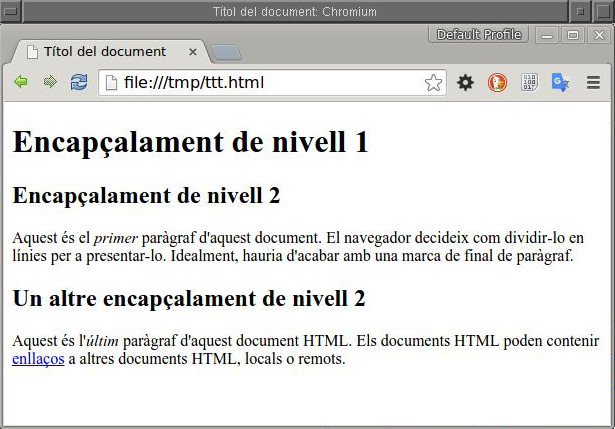
\includegraphics[scale=0.5]{vista-chromium.jpg} \end{center} \caption{El documento XHTML de la figura~\protect\ref{fg:HTML}, visto a través de un navegador de Internet.} \label{fg:HTMLnav} \end{figure} 

El documento XHTML que se muestra en la figura~\ref{fg:HTML} se mostraría en un navegador aproximadamente como en la figura~\ref{fg:HTMLnav}. Como puede verse, la primera línea, que empieza con ``\texttt{<!DOCTYPE}'' declara que el documento es un tipo de documento XHTML estándar según la versión 1.0 \emph{estricta} de XHTML (hay varias versiones). En la tercera línea, la etiqueta ``\texttt{<html>}'' indica el comienzo del documento XHTML, y la etiqueta ``\texttt{</html>}'' del final indica el final del documento. Dentro del elemento \texttt{html} encontramos dos elementos: \texttt{head} (el \emph{encabezamiento}) y body \texttt{} (el \emph{cuerpo} del documento). Dentro del encabezamiento, un elemento \texttt{meta} que no tiene contenido (fijaos cómo se abre y se cierra al mismo tiempo) indica, a través de dos asignaciones del tipo \emph{atributo}\texttt{="}\emph{valor}\texttt{"}, que el \emph{juego de caracteres} que usa el documento es el ISO-8859-1, el más común en Europa occidental.\footnote{Para escribir documentos en \emph{checo} o en \emph{coreano}, habría que cambiar parte del valor del atributo \texttt{content} porque la codificación ISO-8859-1 no permite escribir en estos idiomas.} Dentro de \texttt{head} también encontramos el elemento \texttt{title}, que contiene un título que se presentará, cuando se abra el documento con un navegador, en la barra del navegador, \emph{pero no como parte del texto del documento}. Dentro de \texttt{body} vemos encabezamientos de nivel 1 (\texttt{h1}), encabezamientos de nivel 2 (\texttt{h2}), párrafos (\texttt{p}), partes del texto destacadas (\texttt{em}), y enlaces (\texttt{a}). La tabla~\ref{tb:15etiq} describe algunas de las etiquetas más importantes que se usan en XHTML. 

Cuando estamos mirando un documento HTML con un navegador, podemos ver las etiquetas HTML que lo formatean si seleccionamos la opción ``ver fuente HTML'' (``view HTML source'') o similar que hay normalmente en el menú ``ver'' (``view''). 

\begin{table} \begin{center} \begin{tabular}{l|p{3.2cm}|p{4.3cm}} \hline\hline \textsc{Element} &\textsc{Descripción} &\textsc{Más información} \\ \hline

\texttt{<html>}\ldots\texttt{</html>} &Contiene todo el documento &\\ \hline

\texttt{<head>}\ldots\texttt{</head>} &Encabezamiento &\\\hline \texttt{<body>}\ldots\texttt{</body>} &Cuerpo &\\\hline \texttt{<meta}\ldots\texttt{/>} &Información sobre el documento &El elemento está vacío \\\hline \texttt{<title>}\ldots\texttt{</title>} &Contiene el título del documento &\\\hline \texttt{<br/>} &Salto de línea forzado &El elemento está vacío. \\\hline \texttt{<h1>}\ldots\texttt{</h1>} &Encabezamiento de nivel 1 &\\\hline \texttt{<h2>}\ldots\texttt{</h2>} &Encabezamiento de nivel 2 &\\\hline \(\cdots\) &\(\cdots\) &\(\cdots\) \\\hline \texttt{<h6>}\ldots\texttt{</h6>} &Encabezamiento de nivel 6 &\\\hline \texttt{<p>}\ldots\texttt{</p>} &Párrafo &\\\hline \texttt{<ul>}\ldots\texttt{</ul>} &Lista sin numerar &Contiene elementos \texttt{li} \\\hline \texttt{<ol>}\ldots\texttt{</ol>} &Lista numerada &Contiene elementos \texttt{li} \\\hline \texttt{<li>}\ldots\texttt{</li>} &Elemento de lista &Puede contener otra lista en su interior. \\\hline \texttt{<em>}\ldots\texttt{</em>} &Énfasis &\\\hline \texttt{<strong>}\ldots\texttt{</strong>} &Énfasis fuerte &\\\hline \texttt{<code>}\ldots\texttt{</code>} &Ejemplo de código &\\\hline \texttt{<a}\ldots\texttt{>}\ldots\texttt{</a>} &``Ancla'' &Si lleva un atributo \texttt{href="}URI\texttt{"}, el texto entre ``\texttt{<a}\ldots\texttt{>}'' y ``\texttt{</a>}'' funciona como un enlace al documento que hay en el URI.\\\hline \texttt{<img}\ldots\texttt{/>} &Imagen &El atributo \texttt{src="}URI\texttt{"} indica la dirección donde está la imagen. El atributo \texttt{alt="}\emph{texto}\texttt{"} describe la imagen con palabras. El elemento está vacío.\\\hline \end{tabular} \end{center} \caption{Algunos elementos básicos de XHTML, la versión XML de HTML.} \label{tb:15etiq} \end{table} 

\subsection{Otros formatos basados en XML} Hoy en día se han popularizado los formatos de documentos basados en XML. Algunos de los formatos basados en XML que interesan a los traductores son: el formato TMX (\emph{translation memory exchange}) que se usa para el intercambio de memorias de traducción (ficheros con extensión \texttt{.tmx}, véase el capítulo~\ref{se:memtrad}), el formato TBX (\emph{termbase exchange}) para el intercambio de bases de datos terminológicas (ficheros con extensión \texttt{.tbx}, véase el capítulo~\ref{se:basesdades}) y el formato XLIFF (\emph{XML localization interchange file format}). Este último es un formato creado para la estandarización del formato empleado por las diversas herramientas que se utilizan durante el proceso de \emph{localización} de un producto (véase el capítulo~\ref{se:memtrad}).\footnote{La \emph{localización} se puede definir como el proceso de adaptación de un producto a los usos de una región específica del mundo.} 

Además de los formatos descritos en el párrafo anterior hay dos formatos usados por los procesadores de textos más modernos que están basados en XML. Estos formatos son OpenDocument y Office Open XML. 

\subsubsection{OpenDocument} OpenDocument es un formato de archivos abierto y estándar para almacenar, entre otros, textos (ficheros con extensión \texttt{.odt}) hojas de cálculo (ficheros con extensión \texttt{.ods}) y presentaciones (ficheros con extensión \texttt{.odp}). Este formato es el empleado por defecto por las aplicaciones ofimáticas LibreOffice y Openoffice.org y consiste en varios documentos XML ---para el contenido, los estilos usados en el documento, etc.--- comprimidos con ZIP.\footnote{ZIP es un formato para el almacenamiento de ficheros comprimidos; los ficheros de este tipo suelen tener la extensión \texttt{.zip}.} 

\subsubsection{Office Open XML} Office Open XML, también conocido como OOXML u OpenXML, es otro formato estándar ---impulsado por Microsoft--- basado en XML que se utiliza para almacenar textos (ficheros con extensión \texttt{.docx}), hojas de cálculo (ficheros con extensión \texttt{.xlsx}) y presentaciones (ficheros con extensión \texttt{.pptx}). Igual que OpenDocument, un archivo OpenXML consiste en varios documentos XML comprimidos con ZIP. 

\section{Otros formatos} \subsection{RTF} \label{s3:RTF} 

RTF (\emph{rich text format}, es decir, \emph{formato de texto rico}) fue un formato impulsado por la empresa Microsoft para facilitar el intercambio de documentos entre procesadores de textos manteniendo el formato, y que todavía se usa a veces. RTF también tiene etiquetas, que empiezan normalmente por una barra invertida (\texttt{\textbackslash}); pero los ámbitos de acción de las etiquetas están delimitados por llaves (``\texttt{\{\ldots\}}'') en vez de por parejas de etiquetas; por ejemplo, un segmento en negritas se indica con ``\verb+{\b+\ldots\verb+}+'', mientras que en HTML se usa ``\verb+<B>+\ldots\verb+</B>+''. La figura~\ref{fg:RTF} muestra parte de un documento RTF, en la que se ven algunas instrucciones del encabezamiento (empezando por ``\verb+{\rtf1+...'') y donde también se observa la manera especial como se codifican algunos caracteres. 

\begin{figure}
\begin{center}
\begin{verbatim}
{\rtf1\ansi\ansicpg1252
\end{verbatim}
[\ldots]
\begin{verbatim}
\par
{\b T\`edtol en negretes}\par
Text del par\`a0graf en lletra normal amb alguns incisos 
{\i en cursives} i una marca de final de par\`a0graf al 
final.\par  
Els car\`a0cters que no pertanyen a l'ASCII est\`a0ndard 
s'indiquen amb codis especials (en aquest cas s'ha usat 
ANSI, amb {\i codepage} 1252, com es veu al principi del 
document), com per exemple en el mot 
{\i ling\'fc\'edstica}.\par
\end{verbatim}
[\ldots]
\end{center}
\caption{Parte de un documento de texto en format RTF.} \label{fg:RTF} \end{figure} 

\subsection{PDF} PDF (del inglés \emph{portable document format}, formato portable de documento) es otro formato desarrollado para capturar completamente las características presentacionales de los documentos. En PDF, el documento se muestra exactamente con la misma apariencia independientemente del ordenador, sistema operativo o aplicación que se use para verlo. Los documentos PDF pueden almacenar, además del texto, tipo de letra, gráficos, sonidos, etc. Este formato fue impulsado en los años noventa por la empresa Adobe, que ofrece en la actualidad un programa gratuito\footnote{pero no libre ni de código fuente abierto} denominado Adobe Acrobat Reader DC--- para visualizar los documentos;\footnote{Hay alternativas libres y de código fuente abierto como por ejemplo Sumatra PDF, Evince, Okular, etc. Incluso los mismos navegadores vienen ya con visores de PDF.} para crearlos podemos usar programas especializados o cualquier procesador de textos que permita \emph{exportar} (realmente \emph{imprimir}) nuestro documento a PDF. 

\section{Procesadores de textos}\label{ss:proctext} Un \emph{procesador de textos} es un programa que permite crear y modificar documentos de texto informatizados. También se  pueden usar \emph{editores}: la diferencia entre un procesador de textos y un \emph{editor} es que este último programa es un procesador de textos planos (sin información de formato, etc.) que normalmente se usa para preparar textos en algún lenguaje artificial (por ejemplo, programas escritos en algún lenguaje de programación) que servirán de entrada para otro programa, o textos muy sencillos donde el formato no es crucial, como un mensaje electrónico sencillo. 

El procesamiento de textos también se denomina \emph{tratamiento de textos} (paralelamente al francés, \emph{traitement textes}). En inglés, el énfasis es sobre las palabras: \emph{word processing}. 

Por supuesto, esta sección no pretende instruir en el uso de ningún procesador de textos concreto, sino que quiere describir brevemente algunas características comunes a los procesadores de textos que se usan en la actualidad. De hecho, el uso de los procesadores de texto se aprende mucho mejor en el laboratorio; además, en vista del hecho de que los procesadores de textos cambian constantemente, quizás es mejor no aprender a usar un procesador concreto sino a buscar en cada procesador las herramientas que necesitamos. Esto es posible porque la mayor parte de los procesadores van provistos de manuales o de sistemas de ayuda en línea; algunos tienen incluso ``asistentes'' que observan lo que hace la persona usuaria y le sugieren ---con más o menos fortuna--- posibles acciones en cada momento. 

En cuanto a la \emph{apariencia} del programa, la mayor parte de los procesadores de texto se manifiestan básicamente como una o varias ventanas, cada una de las cuales muestra una sección de alguno de los documentos de texto informatizados que estamos creando y modificando (los documentos que tenemos \emph{abiertos}). La tendencia actual favorece que el texto se muestre tan parecido como sea posible a la versión impresa que se  producirá, en cuanto a formato, tipo de letra, etc.\ (en inglés, este concepto de fidelidad visual se resume con la palabra {\em wysiwyg}, hecho con las siglas de ``what you see is what you get'', es decir, ``lo que veis es lo que obtendréis''); la sección~\ref{s3:problema_wysiwyg} describe algunos problemas derivados de esta tendencia. 

En cuanto a la \emph{operación}, los procesadores de texto asumen que la mayor parte de los caracteres que tecleamos se tienen que insertar detrás del carácter que actualmente se encuentra destacado con una marca llamada {\em cursor} de texto (puede ser diferente del cursor o apuntador que indica la posición virtual del ratón en la pantalla), o bien lo tienen que sobrescribir. Sin embargo, se reservan determinadas teclas (algunas sencillas, y otras en combinación con las teclas especiales ``Alt'' o ``Control'') para hacer operaciones, algunas muy básicas como, por ejemplo, mover el cursor de texto o borrar caracteres y otras más complejas, como, por ejemplo, pegar un bloque de texto que habíamos borrado previamente o guardar el texto completo en el disco.\footnote{Estas teclas y combinaciones de teclas que permiten un acceso rápido a operaciones rutinarias se suelen denominar en inglés \emph{hotkeys}; por ejemplo, en Windows, la combinación control--X recorta el texto seleccionado, la combinación control--V inserta un texto previamente recortado, etc.} Pero muchas de estas operaciones, conjuntamente con otras que no se usan tan a menudo, también están accesibles mediante \emph{menús}; los nombres de estos menús suelen estar situados típicamente en la parte de arriba de la ventana: si se  hace clic con el ratón, se despliegan y nos muestran las opciones que contienen, que podemos elegir con el ratón. 

\paragraph{Sobre la búsqueda de palabras.} Algunos procesadores de textos permiten buscar usando las llamadas \emph{expresiones regulares}, que permiten, mediante caracteres especiales llamados \emph{comodines} (inglés \emph{wildcards}), buscar todas las palabras y todas las porciones de texto que siguen un patrón determinado. Por ejemplo, una búsqueda con la expresión regular \texttt{pres*a} encontraría las palabras \emph{prea}, \emph{presa}, \emph{pressa}, \emph{presssa}, etc., o la expresión regular \texttt{<[\^{}>]+>} que encontraría todas las etiquetas del estilo de XML, puesto que empiezan por \texttt{<}, tienen uno o más (\emph{+}) caracteres que \emph{no} (\texttt{\^}) son \texttt{>}, y acaban con \texttt{>}. Para saber más sobre expresiones regulares podéis consultar la página de la Wikipedia \url{https://es.wikipedia.org/wiki/Expresi%C3%B3n_regular}
.
% A més de l'accés als menús, hi ha operacions que normalment es fan amb
% el ratolí: una de les més importants és \emph{marcar} o
% \emph{seleccionar} una porció de text per a alguna operació posterior
% (per exemple, copiar-la o modificar-ne el tipus de lletra);
% típicament, es fa prement el botó principal del ratolí en un extrem
% del text que volem marcar i, anant, sense soltar-lo, a l'altre extrem.
% Heus ací algunes de les operacions bàsiques que es poden fer amb un
% processador de textos, organitzades de manera similar als menús que
% trobarem en un processador de text:
% \begin{itemize}
% \item Operacions amb fitxers:
%      \begin{itemize}
%      \item \emph{crear} un nou document de text;
%      \item \emph{obrir} un fitxer de document existent en el disc per
%        a treballar-hi;
%      \item \emph{guardar} el document en curs en un fitxer amb el
%        mateix nom i en el mateix format que tenia quan el vam obrir;
%      \item guardar el document en curs amb un altre nom o en un altre
%        format, per exemple el d'un altre processador de textos ({\em
%          guardar com});
%      \item \emph{imprimir} el document actual;
%      \item fer una \emph{presentació preliminar} en pantalla del
%        document tal com quedarà imprés (quan no és possible una
%        presentació completament \emph{wysiwyg})
%      \item \emph{eixir} del processador de textos.
%      \end{itemize}
%    \item Operacions d'edició. A més de les operacions que només es fan
%      des del teclat o amb el ratolí, com ara inserir un caràcter,
%      esborrar-lo, moure'ns pel text, o marcar-hi un passatge, hi ha
%      operacions de modificació del text molt importants que estan
%      accessibles en el menú d'\emph{edició}:
%      \begin{itemize}
%      \item esborrar (\emph{retallar}) la part marcada;
%      \item \emph{copiar} la part marcada a un \emph{portapapers} (una
%        memòria intermèdia) per a usar-la posteriorment;
%      \item inserir (\emph{enganxar} o \emph{apegar}) el contingut del
%        portapapers en un punt del document actual;
%      \item \emph{desfer} o invertir l'última operació (hi ha
%        processadors de text que recorden un nombre considerable
%        d'operacions bàsiques i permeten desfer-ne més d'una, en ordre
%        invers, per descomptat; altres només en recorden l'última
%        operació).
%      \end{itemize}
%    \item Operacions de cerca i substitució:
%      \begin{itemize}
%      \item \emph{buscar} una determinada paraula o seqüència de
%        caràcters en el text;\footnote{Alguns programes permeten buscar
%          usant les anomenades \emph{expressions regulars}, les quals
%          permeten, mitjançant caràcters especials anomenats
%          \emph{jòquers} (anglés \emph{wildcards}), buscar tots els
%          mots i totes les porcions de text que segueixen un patró
%          determinat. Per exemple, una recerca amb l'expressió regular
%          \texttt{pres*a} trobaria els mots \emph{prea}, \emph{presa},
%          \emph{pressa}, \emph{presssa}, etc., o l'expressió regular
%          \texttt{<[\^{}>]+>} que trobaria totes les etiquetes de
%          l'estil de XML, ja que comencen per \texttt{<}, tenen un o
%          més (\emph{+}) caràcters que \emph{no} (\texttt{\^}) són
%          \texttt{>}, i acaben amb \texttt{>}.}
%      \item repetir l'última recerca;
%      \item buscar una determinada paraula o seqüència de caràcters en
%        el text i \emph{substituir-la} per una altra (interactivament o
%        automàticament).
%      \end{itemize}
%    \item Operacions amb tipus de lletra:
%      \begin{itemize}
%      \item selecccionar la grandària de la lletra (per exemple, en
%        \emph{punts}, 1 polzada = 2,54~cm = 72 punts)
%      \item seleccionar la família tipogràfica (Times, Courier,
%        Helvetica...)
%      \item seleccionar l'estil de la lletra: redona, cursiva, negreta,
%        subíndex, superíndex, etc.
%      \end{itemize}
%    \item Operacions de formatatge (normalment els paràgrafs es
%      formaten sols, sense intervenció de la persona usuària en el
%      procés, segons que el va teclejant):
%      \begin{itemize}
%      \item Seleccionar l'alineació o la justificació de les línies del
%        text (alineades a la dreta, a l'esquerra, centrades, o
%        justificades\footnote{No s'ha de dir \emph{justificat a la
%            dreta}: la justificació és sempre als dos marges al mateix
%          temps; el que s'ha de dir en aquest cas és \emph{alineat a la
%            dreta}.});
%      \item seleccionar el format de la pàgina (grandària del paper,
%        marges inferior, superior, dret i esquerre), etc.  S'ha
%        d'esmentar que moltes operacions de formatatge es poden
%        automatitzar i regularitzar usant els estils
%        (p.~\pageref{pg:estil})
%      \end{itemize}
%    \item Altres eines
%      \begin{itemize}
%      \item demanar una \emph{correcció ortogràfica} del text;
%      \item accedir a un \emph{diccionari de sinònims}, etc.
%      \end{itemize}
% \end{itemize}
\section[Contenido, estructura y presentación]{Contenido, estructura y presentación de los documentos} \label{ss:separac} 

\subsection{El problema \emph{wysiwyg}}\label{s3:problema_wysiwyg} La mayoría de los procesadores de textos actuales son \emph{wysiwyg} en el sentido explicado más arriba: el texto que se edita se presenta gráficamente en la ventana prácticamente igual a como se verá en el papel cuando lo enviemos a la impresora; esto ha facilitado enormemente el acceso de todo el mundo a los procesadores de textos. Pero el esquema \emph{wysiwyg}, completamente generalizado desde mitad de los ochenta, tiene también, como veremos, sus inconvenientes. La persona escritora tiende a centrarse en los atributos \emph{visuales} del texto (tipo y tamaños de letra, márgenes, etc.), puesto que confía en que una buena \emph{presentación} transmitirá a las personas lectoras la estructura \emph{lógica} que la persona escritora tiene en la cabeza. Con el documento, por lo tanto, sólo se guardará esta información de presentación, prácticamente sin ninguna indicación de la estructura lógica de los contenidos. Imaginaos las siguientes situaciones problemáticas: \begin{quote} Vladimir ha decidido que los títulos de sección del informe anual que le han encargado estarán en Helvetica de 14 puntos, negrita y los de subsección en Arial de 12 puntos, negrita cursiva. A su directora no le gustan así y se los ha hecho cambiar a Lucida Sans de 14, negrita y Lucida de 12, negrita sin cursivas. Como el informe tiene que estar acabado para mañana por la mañana, Vladimir se queda en la oficina hasta las 11 de la noche, cambiando uno por uno los tipos de letra de los títulos de secciones y subsecciones. El día siguiente, por la mañana, Marina, la directora, le pasa un documento con una sección más que se tiene que insertar entre la 4 y la 5. Vladimir no puede ir a almorzar: tiene que cambiar los números de secciones y subsecciones a partir de la 5 y repasar si se tiene que cambiar alguna referencia que se haga desde una parte del texto a una sección por su número. \end{quote} 

\begin{quote} Nos han encargado traducir un texto informatizado. En la lengua origen es costumbre poner en \emph{cursivas} tanto las palabras extranjeras (``\emph{Sprachgefühl}'') como los términos cuando se definen por primera vez (``Un \emph{byte} es...''), se sangra la primera línea de todos los párrafos, y los números de sección traen un punto al final (``1.1. Introducción''), pero en la lengua de llegada los términos nuevos van en negritas (``Un \textbf{byte} es ...''), se sangra la primera línea de todos los párrafos excepto la del primer párrafo de una sección, y los números de sección no llevan punto al final (``1.1 Introducción''). El texto ha sido traducido manteniendo las convenciones de la lengua origen: para hacerlo adecuado a la lengua de llegada, nos toca, por un lado, ir mirando uno por uno los segmentos de texto en cursivas, decidir si son definiciones, y cambiarlos a negritas si hace falta; por otro lado, nos toca ir quitando el puntito final de todos los números de sección. \end{quote} 

En estos dos casos, si la persona que escribió los textos sólo codificó información relativa a la presentación visual no podremos evitar hacer los trabajos tediosos descritos. Se podría decir que si quien escribe se deja llevar por la filosofía ``what you see is what you get'' acaba con ``what you see is \emph{all} you get'', es decir, sólo tiene lo que ve. Pero la mayoría de los procesadores de textos \emph{wysiwyg} actuales permiten un cierto nivel de codificación de  la \emph{estructura}, a través de los llamados \emph{estilos}:\footnote{Esta es la denominación usada por \emph{Word} y por los procesadores libres y de código abierto \emph{Openoffice.org} y  \emph{LibreOffice}.} hay \emph{estilos de párrafo} (párrafo del cuerpo de texto, encabezamientos de varios niveles, etc.) y estilos \emph{de carácter} (definiciones, énfasis, énfasis fuerte, texto de ordenador, etc.).\label{pg:estil} A cada estilo se le asignan unas determinadas características de presentación: por ejemplo, los encabezamientos de nivel 2 van en Helvetica de 14 puntos negrita y numerados automáticamente con el número de la sección de nivel 1, un punto y el número de la sección de nivel 2; las definiciones van en negrita y el énfasis en cursiva, etc. El procesador de textos aplica automáticamente las mismas características de presentación \emph{a todos los segmentos del documento} que tienen el mismo estilo. Esto resolvería las situaciones problemáticas explicadas más arriba. 

En el primer problema, si se hubieran usado los estilos como se indica, la numeración y el estilo de las secciones se determinaría automáticamente y sólo habría que indicar (sólo una vez) qué tipo de letra corresponde a los títulos de sección; además se renumerarían automáticamente todas las secciones. Si las referencias de unas secciones a otras se hubieron hecho usando referencias cruzadas simbólicas (muchos procesadores de textos las permiten), también se actualizarían automáticamente. 

En el segundo problema, si el documento hubiera contenido información sobre qué términos son definiciones y cuáles son palabras extranjeras, sólo habría que cambiar el estilo de las definiciones y todas quedarían en negritas. Por otro lado sólo habría que indicar que no es necesario el último punto en los números de sección y todos pasarían automáticamente al formato deseado. 

Estos ejemplos ilustran la conveniencia de que los autores de los documentos se centren más en la estructuración lógica del contenido del documento que escriben. Después, sólo hay que indicar al procesador cuál tiene que ser la presentación de cada elemento de esta estructura lógica y obtendremos la presentación deseada. 

\subsection{Hojas de estilo} En XML y HTML, esta separación entre la estructura del contenido y la presentación de un documento se ejecuta a través de especificaciones llamadas \emph{hojas de estilo}. Uno de los tipos más sencillos de hojas de estilo son las llamadas hojas de estilo en cascada\footnote{Más información en \url{http://www.w3c.org/Style/CSS/}.} (CSS, \emph{cascaded style sheets}) que se usan sobre todo con navegadores y HTML, aunque también se pueden usar para presentar XML directamente en los navegadores. 

Las hojas de estilo CSS asignan características de presentación a cada
elemento del documento. Por ejemplo, la orden CSS 
\begin{verbatim}
h2 {   display : block ;
       font-size : large ;
       font-family : sans-serif ;
       text-align : left ;
       margin-top: 0.2cm ;
       margin-bottom : 0.2cm ; }
\end{verbatim}
indica que todos los encabezamientos de segundo nivel (\texttt{h2}) de (X)HTML se visualizan (\texttt{display}) como bloques de texto separado (\texttt{block}), con un tamaño de letra (\texttt{font-size}) grande (\texttt{large}) de la familia \emph{sans serif}, alineado (\texttt{text-align}) a la izquierda, y con márgenes superior e inferior de 0,2 cm. 

Las hojas de estilo se pueden usar también para visualizar documentos
XML directamente en los navegadores más recientes. Por ejemplo,
podemos hacer que la presentación visual del mensaje de correo
electrónico de la figura~\ref{fg:faxXML} tenga un encabezamiento con
el texto ``\emph{Mensaje de correo}'' centrado, grande y en negritas
con esta orden CSS (con comentarios entre \texttt{/*} y  \texttt{*/}): 
\begin{verbatim}
EMAIL:before {                     /*Antes del EMAIL*/
   content : "Mensaje de correo" ; /*El texto deseado*/
   display : block ;               /*como un bloque*/
   font-weight : bold ;            /*en negrita*/
   text-align : center ;           /*centrado */
   font-size : x-large ;           /*y con letra extragrande*/
}
\end{verbatim}

En el caso de las hojas de estilo CSS, el esquema de uso es el que se indica en la figura~\ref{fg:CSS}: el navegador lee el documento HTML o XML,  aplica los estilos de la hoja CSS, y genera una presentación. La hoja de estilo CSS puede estar en el mismo fichero que el documento HTML o XML, o en un fichero externo. 

\begin{figure} $$ \left. \begin{array}{rcl} \mbox{\textsf{Documento XML o HTML}} &\to \\ \mbox{\textsf{Hoja de estilo CSS}} &\to \\ \end{array} \right. \mbox{\framebox{\parbox{1.8cm}{\textsf{Navegador}}}} \to \mbox{\parbox{1.8cm}{\textsf{Presentación}}} $$ \caption{Presentación de documentos XML y HTML con hojas de estilo CSS.} \label{fg:CSS} \end{figure} 

Para la presentación de documentos XML, existe un lenguaje de programación de hojas de estilo mucho más potente que CSS llamado XSL\footnote{Más información en \url{http://www.w3c.org/Style/XSL/}.} (\emph{extended stylesheet language}) que permite \emph{transformar} un documento XML (con etiquetas que  indican la estructura del contenido) en otro documento XML, HTML o de cualquier otro formato (Postscript, PDF, RTF, etc.), por ejemplo, para presentarlo visualmente (véase la figura~\ref{fg:XSL}). Los navegadores más recientes ya son capaces de aplicar hojas de estilo XSL a páginas \emph{web} escritas en XML y presentarlas cómo si estuvieron escritas originalmente en HTML. 

Este tipo de presentación visual no es la única transformación posible que podemos obtener con hojas de estilo: como se muestra en la figura~\ref{fg:braille}, para un mismo documento XML podemos generar un conjunto de \emph{vistas} de su contenido en diferentes medios (\emph{media}) sólo usando la hoja de estilo adecuada. 

\begin{figure} $$ \left. \begin{array}{rcl} \mbox{\textsf{Documento XML}} &\to \\ \mbox{\textsf{Hoja de estilo XSL}} &\to \\ \end{array} \right. \mbox{\framebox{\parbox{2.1cm}{\textsf{Procesador de XSL}}}} \to \mbox{\parbox{2.1cm}{\textsf{Documento (XML, HTML, etc.) }}} $$ \caption{Transformación de documentos XML con hojas de estilo XSL.} \label{fg:XSL} \end{figure} 

\begin{figure} \centering \setlength{\unitlength}{1cm} \begin{picture}(11,6)(0,1.5) \put(0,1){\makebox(3,2){\sf Fichero de sonido}} \put(4,1){\makebox(3,2){\sf Documento Braille}} \put(8,1){\makebox(3,2){\sf Documento para móviles}} \put(1.5,2.6){\makebox(0,0){\LARGE \twonotes}} \put(5.5,2.6){\makebox(0,0){\LARGE \Printer}} \put(9.5,2.6){\makebox(0,0){\LARGE \Mobilefone}} \put(0,4){\framebox(3,1){\sf Hoja de estilo 1}} \put(4,4){\framebox(3,1){\sf Hoja de estilo 2}} \put(8,4){\framebox(3,1){\sf Hoja de estilo 3}} \put(4,6){\makebox(3,2){\sf Documento XML}} \put(5.5,6.5){\line(0,-1){0.75}} \put(1.5,5.75){\line(1,0){8}} \put(1.5,5.75){\vector(0,-1){0.5}} \put(5.5,5.75){\vector(0,-1){0.5}} \put(9.5,5.75){\vector(0,-1){0.5}} \put(1.5,4){\vector(0,-1){1}} \put(5.5,4){\vector(0,-1){1}} \put(9.5,4){\vector(0,-1){1}} \end{picture} \caption{Obtención de tres presentaciones diferentes de un único documento XML mediante hojas de estilo.} \label{fg:braille} \end{figure} 

\subsection{Accesibilidad} En casi toda la discusión anterior hemos hablado de presentación refiriéndonos siempre a un medio visual, de forma que hemos excluido, por ejemplo, a las personas que tienen discapacidades o limitaciones relacionadas con el sentido de la vista (pueden no ver nada o ver muy mal, o sufrir ataques epilépticos cuando ven una imagen que cambia rápidamente de color). Cuando presentamos un documento visualmente, intentamos que la representación visual de las diversas partes del documento comuniquen la estructura lógica del contenido a la persona lectora, pero, ¿cómo presentamos la estructura lógica de un documento a una persona ciega? Mecanismos como los tipos o tamaños de letra o la forma o el alineamiento visual de los párrafos, listas o tablas no le sirven; esta persona quizás quiere acceder a los documentos mediante un tablero Braille (una especie de pantalla táctil donde se forman los signos del alfabeto de los invidentes, véase la figura~\ref{fg:braille}) o mediante un sistema de síntesis de voz que lea la página en voz alta. 

Si quien ha escrito el documento sólo ha codificado la estructura lógica que tenía en su cabeza mediante indicadores visuales de formato (negritas o cursivas para el énfasis, párrafos de una línea en letra más gorda para títulos, etc.) será difícil transformar este formato para otra presentación. 

\begin{figure} \centering

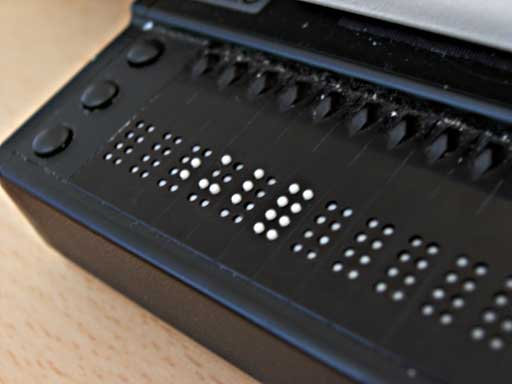
\includegraphics[scale=0.5]{Refreshable_Braille_display.jpg} \caption{Tablero braille (imagen tomada de la entrada \emph{Refreshable Braille Display} de la Wikipedia en inglés)} \end{figure} 

Pero no sólo las personas con discapacidades visuales pueden tener problemas; quien lee un documento lo puede estar haciendo a través de una pantalla de texto (no gráfica) o pequeña (como la de un teléfono móvil), o a través de una conexión muy lenta a la red, o puede estar en una situación en la cual sus ojos estén ocupados (por ejemplo, cuando conduce un vehículo). La presentación de documentos en estos medios tiene problemas similares. 

Si el énfasis en el documento ha sido almacenado como énfasis y no con letra negrita o cursiva, si los títulos de sección están indicados como tales y no porque son párrafos de una única línea en negritas gordas, será mucho más fácil transformarlo para presentarlo en un medio no visual o en una pantalla reducida o limitada, por ejemplo, usando \emph{hojas de estilo} especialmente concebidas para la presentación \emph{aural} (sonora), \emph{táctil} (Braille), etc. 

La separación de la estructuración del contenido, por un lado, y de los mecanismos de presentación del documento, por otro, facilita la \emph{accesibilidad} al documento a través de varios medios a personas discapacitadas o en situaciones especiales. 

\begin{persabermes}{tecnologías auxiliares para la generación de textos} \paragraph{Reconocimiento automático del habla.} El \emph{reconocimiento automático del habla} (RAH) se puede definir como la producción de textos informatizados ---en \emph{tiempo real}, es decir, tan instantáneamente como sea posible--- a partir de la voz humana (véase \citealt{samuelson-brown96b}). El RAH de propósito general está todavía muy lejos de ser perfecto, y, de hecho, es todavía un campo de investigación activo, aunque recientemente se ha incorporado bastante satisfactoriamente a dispositivos como por ejemplo teléfonos móviles (por ejemplo, los dispositivos con sistema operativo Android permiten hacer búsquedas por voz). En cambio, el RAH para un propósito específico (por ejemplo, la consulta telefónica de horarios de trenes o de las condiciones del tráfico) está mucho más avanzado. La mayor parte de la inversión de la comunidad internacional en RAH es, por razones obvias, sobre el inglés. 

El RAH genera texto a partir de la voz recogida a través de un micrófono utilizando un dispositivo de captura para digitalizarla y después un sistema de reconocimiento automático de la voz (\emph{automatic speech recognition}) para detectar fonemas, sílabas o palabras completas (depende del sistema concreto) y traducirlas posteriormente a un texto informatizado. Hay sistemas de reconocimiento {\em independientes del hablante} y sistemas \emph{dependientes del hablante} (los últimos normalmente tienen que ser \emph{entrenados} por la persona antes de su uso). El RAH es especialmente difícil por la gran variabilidad acústica que presentan los fonemas: \begin{itemize} \item según el contexto articulatorio (por ejemplo, no es igual el sonido del fonema palatal catalán representado por el dígrafo \emph{ig} en ``passeig curt'' ---sordo--- que en ``passeig allargat'' ---sonoro---); \item según el hablante (cada persona tiene unos órganos fonadores de forma diferente ---acústicamente diferentes--- y procesos de producción del habla diferentes ---por ejemplo, hay quién habla más despacio y quien habla muy de prisa---); \item según el dialecto del hablante (por ejemplo, los valencianos hacemos africadas las \emph{j} que en catalán central son palatales fricativas sonoras). \item según el estado emocional del hablante, etc. \end{itemize} Es un hecho muy establecido que, para superar estas dificultades, los humanos hacemos un uso muy intensivo de los conocimientos lingüísticos que tenemos sobre el idioma que estamos escuchando y del contexto comunicativo: así, si oímos decir ``\emph{percà nom} passes l'\emph{antre xoc} de \emph{craus}?'' a un amigo cuando vemos que no puede abrir el coche, entendemos perfectamente que nos quiere decir \emph{¿Por qué no me pasas el otro juego de llaves?}, o si oímos decir en voz alta ``mu han dim moltis baltes'' es muy probable que entendamos claramente ``me lo han dicho muchas veces'' a pesar de los cambios fonéticos, puesto que inconscientemente buscamos la interpretación correcta más cercana a lo que hemos oído (en el contexto concreto en que se diga la frase). Considerad este doblete inglés clásico sobre el tema: \emph{people can easily recognize speech} no es muy diferente de {\em people can easily wreck a nice beach}; otro doblete lo forman las expresiones \emph{sax and violins on TV} y la más verosímil \emph{sex and violence on TV}. Los resultados del RAH son especialmente dependientes de las particularidades lingüísticas de la lengua involucrada y el éxito depende de la existencia de un buen \emph{modelo de lengua} ---rápido y conciso, es decir, computacionalmente eficiente--- que simule la parte no contextual de la comprensión humana y permita obtener el texto más probable en un idioma determinado a partir del texto en bruto producido por el sistema de RAH. La mayor parte de los sistemas usan vocabularios grandes y modelos estadísticos. 

\paragraph{Reconocimiento automático de textos escritos.} El \emph{reconocimiento automático de textos escritos} (RATE) se puede definir como la producción de textos informatizados a partir de textos manuscritos o tipografiados. En el caso de textos tipografiados la tarea es mucho más sencilla; en el caso de manuscritos, la complejidad es comparable a la del reconocimiento del habla. 

El RATE genera un texto informatizado a partir de un documento impreso, usando un escáner (en inglés \emph{scanner}) y un programa de reconocimiento óptico (también se conoce como {\em automático}) de caracteres (OCR, \emph{optical character recognition}). Primeramente, el documento impreso es leído (escaneado) usando el escáner, y se  genera un fichero que  contiene la imagen digital (por ejemplo, una parrilla muy fina de cuadrados blancos y negros). Después, el programa de OCR lee la página, descubre donde están los párrafos, las líneas y, finalmente, los caracteres concretos, y los transforma en un texto informatizado (normalmente bastante imperfecto, especialmente si es manuscrito). Como en el caso del reconocimiento del habla, es crucial el uso de información sobre el idioma concreto (diccionarios, estadística sobre las secuencias de letras) para corregir los errores del OCR. Por ejemplo, si un programa de lectura automática de textos produce por error el texto ``4ixò 6s uua mcrda'', huelga decir que lo leemos sin demasiados problemas, a pesar de los errores en todas las palabras; esto es gracias a nuestros conocimientos sobre las secuencias de letras comunes en catalán. 

\mbox{} \end{persabermes} 

\section{Cuestiones y ejercicios} \begin{enumerate} \item Para validar un documento XML necesitamos {\ldots} \begin{enumerate} \item {\ldots} otro documento XML, este último con las marcas sin contenido. \item {\ldots} una hoja de estilo CSS. \item {\ldots} una definición de tipo de documento (DTD). \end{enumerate} 

\item ¿Cómo se indica en una DTD que el elemento \texttt{teixit} contiene opcionalmente los elementos \texttt{grandaria} y  \texttt{color} en este orden? \begin{enumerate} \item \verb|<!MARK teixit grandaria, color #OPTIONAL>| \item \verb|<!MARK teixit (grandaria?,color?)>| \item \verb|<!ELEMENT teixit (grandaria?,color?)>| \end{enumerate} 

\item Un documento XML es \emph{válido} {\ldots} \begin{enumerate} \item {\ldots} si sólo usa los nombres de elementos definidos en la DTD; el resto de las directrices de la DTD sólo sirven para hacer documentos \emph{bien formados}. \item {\ldots} si sólo usa las marcas válidas de los documentos HTML. \item {\ldots} si sigue las reglas de la DTD cuando incluye un elemento dentro de otro y, además, no incluye ningún elemento no definido en la DTD. \end{enumerate} 

\item Un texto informatizado se caracteriza principalmente {\ldots} \begin{enumerate} \item {\ldots} por su formato, por un lado, y por el juego de caracteres con que está codificado, por otro. \item {\ldots} por la versión del sistema operativo y el procesador de textos con que ha sido escrito. \item {\ldots} por la hoja de estilo que indica los aspectos estéticos de su presentación. \end{enumerate} 

\item ¿Qué hace que el siguiente fragmento de XML esté \emph{mal formado}? \begin{center}\verb|<tit int=hi>Zjuknim agarnow</tit>|\end{center} \begin{enumerate} \item Entre \verb|tit| y \verb|>| no puede haber nada. \item La etiqueta \verb|tit| no es válida en XML; tendría que ser \verb|title|. \item Si hay algún atributo, el valor tiene que ir entre comillas. \end{enumerate} 

\item Si en una DTD encontramos las reglas 
\begin{verbatim} 
<!ELEMENT taula (capçalera?,fila+)> 
<!ELEMENT fila (casella*)> 
<!ELEMENT casella (#PCDATA|taula)*> 
\end{verbatim}
¿cuál de las tres situaciones siguientes es válida de acuerdo con esta DTD? \begin{enumerate} \item \verb|<taula></taula>| \item \verb|<taula><fila><casella>zz<taula><fila></fila></taula>zz| \verb|</casella><fila></taula>| \item \verb|<taula><fila><casella>zz</casella><casella>ww</casella>| \verb|</fila></taula>| \end{enumerate} 

\item ¿Qué indica el fragmento \texttt{encoding="\ldots"} en la primera línea (\texttt{<?xml\ldots?>}) de un documento XML? \begin{enumerate} \item La versión de XML. \item Dónde está la DTD necesaria para validarlo. \item Cuál es el juego de caracteres que usa el documento XML. \end{enumerate} 

\item Cuántos bytes ocupa el segmento de XML siguiente: \begin{center}\verb|<qq>ww</qq>|\end{center} \begin{enumerate} \item 11 como mínimo, dependiendo de la codificación. \item 11, independientemente de la codificación. \item 4 exactamente. \end{enumerate} 

\item Cuando las marcas de formato sólo especifican el \emph{contenido} de un documento (identificando las partes y la estructura de cada una), ¿cómo se asigna una \emph{presentación} determinada al documento? \begin{enumerate} \item Con una o más hojas de estilo. \item Con una codificación de caracteres (p.e., Unicode o ISO-8859-1). \item No se  puede asignar presentación. \end{enumerate} 

\item ¿Qué se conserva de ASCII en los sistemas de codificación de caracteres más avanzados como Unicode UTF-8, ISO-8859-1 (\emph{Latin-1}), etc.? \begin{enumerate} \item Los caracteres y sus números de código. \item Los caracteres, pero con números de código diferentes. \item No  queda nada. Se ha reorganizado toda la codificación. \end{enumerate} 

\item Estamos en Eslovaquia, donde se usa la codificación de caracteres ISO-8859-2 (\emph{Latin-2}). Desde Alacant, nos envían un documento de texto plano, escrito con la codificación ISO-8859-1 (\emph{Latin-1}) y lo abrimos como si fuera ISO-8859-2 (\emph{Latin-2}). ¿Qué pasa? \begin{enumerate} \item No vemos bien ninguna letra: todo son símbolos extraños e ininteligibles. \item Vemos bien todas las letras excepto las acentuadas, las que llevan diéresis, la  \emph{ñ} o la \emph{ç}: en su lugar aparecen otros símbolos o letras típicas de las lenguas de Europa del Este. \item Vemos bien todas las letras excepto las acentuadas, las que llevan diéresis, la \emph{ñ} o la \emph{ç}: en su lugar aparecen las versiones sin acento, la  \emph{n}  o la \emph{c}. \end{enumerate} 

\item ¿Qué es RTF? \begin{enumerate} \item Un esquema avanzado de codificación de caracteres. \item Un formato abierto de intercambio de memorias de traducción. \item Un formato abierto para intercambiar documentos de texto entre procesadores de textos. \end{enumerate} 

\item Un documento HTML tiene un enlace con el texto ``Más información'' y con URI de destino \verb|http://www.detalls-e.com/mes.html|. ¿Cómo es este enlace en HTML? \begin{enumerate} \item \verb|<a href="http://www.detalls-e.com/mes.html">Más información</a>| \item \verb|<a href="Més informació">http://www.detalls-e.com/mes.html</a>| \item \verb|<a htxt="Més informació" href="http://www.detalls-e.| \verb|com/mes.html">| \end{enumerate} 

\item ¿Dónde va el título de un documento HTML (el que se muestra en \emph{la barra} del navegador)? \begin{enumerate} \item En un elemento \verb|title| dentro de \verb|head|. \item En un elemento \verb|title| dentro de \verb|body|. \item En un elemento \verb|h1| dentro de \verb|head|. \end{enumerate} 

\item Si los caracteres de un texto están codificados usando el juego de caracteres ISO-8859-1 (\emph{Latin-1}), ¿qué códigos tienen las letras de la \verb|A| a la \verb|Z|? \begin{enumerate} \item Depende del formato del texto (HTML, etc.). \item Los mismos que en la codificación ASCII. \item Los que tenían en la codificación ASCII más 128. \end{enumerate} 

\item ¿Cuántos bytes ocupa como mínimo el siguiente fichero HTML? \begin{center} \verb|<html><body><p>Texto.</p></body></html>| \end{center} \begin{enumerate} \item 11 \item 39 \item 76 \end{enumerate} 

\item En la codificación de caracteres ISO-8859-1 (\emph{Latin-1}), todos los caracteres acentuados del español o del catalán tienen códigos {\ldots} \begin{enumerate} \item {\ldots} entre 0 y 127. \item {\ldots} entre 128 y 255. \item {\ldots} mayores que 256. \end{enumerate} 

\item Un texto codificado en ISO-8859-1 (\emph{Latin-1}) tiene 1000 caracteres justos (contando los espacios en blanco y los saltos de línea). ¿Cuántos bytes ocupa? \begin{enumerate} \item 1000 exactamente, 1 por carácter. \item 2000 exactamente, 2 por carácter. \item entre 1000 y 2000, entre 1 byte y 2 bytes por carácter. \end{enumerate} 

\item En XML, si se abre un elemento con la marca \verb|<frase>|, ¿con qué marca se cierra? \begin{enumerate} \item Con \verb|</frase>|. \item Con \verb|<frase>|. \item Automáticamente cuando se abre cualquier otro elemento. \end{enumerate} 

\item Si en un documento XML encontramos la situación \begin{center}\verb|<rec><id>Zork</id><addr>Zmeggs</addr></rec>|\end{center} y una DTD define el elemento \verb|rec| con la regla \begin{center}\verb|<!ELEMENT rec (id,up?,addr*)>|\end{center} ¿Puede ser que el documento sea válido según la DTD? \begin{enumerate} \item Depende de cómo sea de estricto el programa validador. \item No, porque esta situación no es válida. \item Sí, si el resto del documento es válido. \end{enumerate} 

\item ¿Qué vemos si abrimos un texto HTML con un editor de textos sencillo como el \emph{Bloc de notas} o \emph{Notepad} de Windows? \begin{enumerate} \item El texto HTML pero sin las marcas entre ``\verb|<|'' y ``\verb|/>|''. \item El texto HTML tal como está hecho por dentro, con las marcas entre ``\verb|<|'' y ``\verb|>|'' y todo. \item Una pantalla en blanco. \end{enumerate} 

\item ¿En que se diferencian dos extensiones de ASCII diferentes? \begin{enumerate} \item En los caracteres asignados a los 256 códigos. \item En los caracteres asignados a los códigos del 0 al 127. \item En los caracteres asignados a los códigos del 128 al 255. \end{enumerate} 

\item Si en una DTD encontramos la regla \begin{center}\verb|<!ELEMENT cv (nom,any?,ob+)>|\end{center} ¿cuál de las tres situaciones siguientes no es válida de acuerdo con esta DTD? \begin{enumerate} \item \verb|<cv><nom>Pere</nom><any>1992</any></cv>| \item \verb|<cv><nom>Pere</nom><ob>Escrits</ob></cv>| \item \verb|<cv><nom>Pere</nom><any>1992</any><ob>Crits</ob><ob>Plors</ob></cv>| \end{enumerate} 

\item En un documento HTML queremos que la frase \emph{este documento} sea un enlace al documento que tiene el URI \verb|http://www.uc.za/t.html|: ¿cuál de las siguientes porciones de HTML es la correcta? \begin{enumerate} \item \verb|<a url="http://www.uc.za/t.html">este documento</a>| \item \verb|<a href="http://www.uc.za/t.html">este documento</a>| \item \verb|<link url="http://www.uc.za/t.html">este documento</link>| \end{enumerate} 

\item El fragmento de documento HTML ``\verb|<strong><em>link</strong></em>|'' tiene un error. ¿Cuál es la causa? \begin{enumerate} \item El nombre de las marcas no es válido, porque no  indica ninguna información sobre el contenido. \item El orden de las marcas de apertura y cierre no es correcto. \item No se ha indicado el valor del atributo \verb|href| del elemento \verb|em|. \end{enumerate} 

\item La longitud media de una palabra en gondavés es de 5,5 caracteres y la edición electrónica de \emph{Gundhawól Vlâj} (``La Voz de Gondàvia''), tiene unas 100.000 palabras diarias como media. Si el gondavés se escribe usando la codificación ISO-8859-1 (\emph{Latin-1}), ¿cuántos ejemplares del diario se pueden guardar en un CD-ROM? \begin{enumerate} \item Más de dos años. \item Un ejemplar sólo. \item Un mes aproximadamente. \end{enumerate} 

\item ¿Cómo se indica en una DTD que el elemento \verb|<fitxa>| contiene obligatoriamente los campos \verb|<nom>| y \verb|<tel>| y, opcionalmente, el campo \verb|<email>|? \begin{enumerate} \item \verb|<!ELEMENT fitxa (nom,tel,email?)>| \item \verb|<!ELEMENT fitxa (nom,tel,email+)>| \item \verb|<!ATTLIST fitxa nom CDATA #required| \newline\verb| tel CDATA #required email CDATA>| \end{enumerate} 

% \item En XHTML (o HTML) hi ha elements buits (sense contingut).
%   Digues en quina d'aquestes tres opcions els dos elements són buits.
%   \begin{enumerate}
%   \item \texttt{h1} i \texttt{meta}.
%   \item \texttt{meta} i \texttt{img}.
%   \item \texttt{meta} i \texttt{head}.
%   \end{enumerate}
\item En XML, ¿que quiere decir \texttt{<mang/>}? \begin{enumerate} \item No quiere decir nada, porque no hay ningún elemento que se llame \texttt{mang}. \item Lo mismo que \texttt{<mang></mang>}. \item No quiere decir nada, porque tendría que ser \texttt{</mang>}. \end{enumerate} 

\item ¿Cuál de estos tres elementos XHTML (o HTML) no puede ir dentro del elemento \texttt{body}? \begin{enumerate} \item \texttt{meta}. \item \texttt{img}. \item \texttt{h1}. \end{enumerate} 

\item Tenemos un documento XML que es válido de acuerdo con una determinada DTD. Borramos un elemento completo (por ejemplo \texttt{<element>text</element>}), que no es el elemento raíz del documento. ¿Cuál de estas tres situaciones no es posible? \begin{enumerate} \item Que el documento XML resultante no sea válido respecto de la DTD. \item Que el documento XML sea válido respecto de la DTD. \item Que el documento XML no sea un documento XML bien formado. \end{enumerate} 

\item En HTML, ¿podemos poner un enlace \texttt{<a href="..."}\texttt{>...</a>} dentro de un elemento de lista \texttt{<li>...</li>?} \begin{enumerate} \item Sí. \item No, porque el documento estaría mal formado. \item No, porque el documento no sería válido. \end{enumerate} 

\item Un fichero de texto escrito en inglés contiene sólo caracteres ASCII. Lo abrimos con un editor y lo guardamos en formato Unicode UTF-8. Ahora ocupa {\ldots} \begin{enumerate} \item {\ldots} el doble de espacio. \item {\ldots} exactamente el mismo espacio. \item {\ldots} la mitad de espacio. \end{enumerate} 

\item Señala el fragmento de HTML que generará el texto más grande: \begin{enumerate} \item \texttt{<h1>Título</h1>} \item \texttt{<h2>Título</h2>} \item \texttt{<h3>Título</h3>} \end{enumerate} 

\item ¿Cómo se llama el juego de caracteres estándar universal, el que asigna un número de código diferente y único a cada uno de los caracteres de cada una de las lenguas del mundo? \begin{enumerate} \item Unicode. \item ISO-8859-1 (\emph{Latin-1}). \item XML. \end{enumerate} 

\item ¿Cuándo es preferible utilizar el juego de caracteres Unicode en lugar del ISO-8859-1 (\emph{Latin-1})? \begin{enumerate} \item Cuando vamos a mezclar texto en diferentes idiomas. \item Cuando un texto en español tiene muchos acentos. \item Cuando el texto sólo se usará en una situación de asimilación. \end{enumerate} 

\item Podemos almacenar correctamente el texto en español ``\emph{La España de charanga y pandereta, cerrado y sacristía, devota de Frascuelo y de María, de espíritu burlón y de alma quita}'' usando el juego de caracteres ASCII? \begin{enumerate} \item Sí, sin problemas. \item Sí, si antes lo hemos convertido a UTF-8. \item No. \end{enumerate} 

\item ¿Cuánto ocupa un fichero de texto que contiene 2000 caracteres pertenecientes al alfabeto español? \begin{enumerate} \item Si se ha codificado en ISO-8859-1 (\emph{Latin-1}), entre 2000 y 4000 bytes. \item Si se ha codificado en ASCII, 2000 bytes. \item Si se ha codificado en UTF-8, entre 2000 y 4000 bytes. \end{enumerate} 

\item Si al visualizar el documento de texto \texttt{noticia.txt} en el navegador  aparecen palabras como \texttt{camiÃ\(^3\)n} e \texttt{Informática}, ¿cuál  puede ser la causa? \begin{enumerate} \item Un error por parte de la persona que ha escrito el documento de texto. \item Que el navegador está usando para leer el documento un juego de caracteres diferente del que se usó al escribirlo. \item Que el documento no es un documento HTML. \end{enumerate} 

\end{enumerate} 

\section{Soluciones} \begin{enumerate} \item (c) \item (c) \item (c) \item (a) \item (c) 

%
\item (c) \item (c) \item (a) \item (a) \item (a) 

%
\item (b) \item (c) \item (a) \item (a) \item (b) 

%
\item (b) \item (b) \item (a) \item (a) \item (c) 

%
\item (b) \item (c) \item (a) \item (b) \item (b) 

%
\item (a) \item (a) \item (b) \item (a) \item (c) 

%
\item (a) \item (b) \item (a) \item (a) \item (a) 

%
\item (c) \item (c) \item (b) \end{enumerate} 

